\section{System Calls}

\begin{frame}{Introducción System Call Interface}
  \begin{itemize}
  \item Los SOs proveen un conjunto de interfaces mediante las cuales un proceso que corre en espacio de usuario interactúa con el Kernel
  \item En UNIX existe un API principal que provee:
  \begin{itemize}
    \item El \alert{API} principal del SO
    \item Librerías standard de C
    \item \alert{Interface para las System Calls}
    \end{itemize} 
  \end{itemize}
\end{frame}

\begin{frame}{POSIX APIs}
  \begin{itemize}
  \item Los SO exponen funcionalidad del Kernel a través de \alert{System Calls} 
  \item Su próposito es proveer una interfaz para que los desarroladores interactuén con el \alert{Kernel}
  \item Los SO Unix exponen esta funcionalidad en forma de \alert{API}
  \item El desarrollador interactúa con el \alert{API} y NO directamente con \alert{System Calls}  
  \item En UNIX por lo general cada función del \alert{API} se corresponde con una \alert{System Call}
  \end{itemize}
  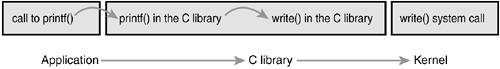
\includegraphics[width=\linewidth]{images/printf.jpg}
\end{frame}

%%% Local Variables: 
%%% mode: latex
%%% TeX-master: "main"
%%% End:
